% This is samplepaper.tex, a sample chapter demonstrating the
% LLNCS macro package for Springer Computer Science proceedings;
% Version 2.20 of 2017/10/04
%
\documentclass[runningheads]{llncs}
%
\usepackage{graphicx}
\graphicspath{ {./img/} }

% Copyright 2017 Sergei Tikhomirov, MIT License
% https://github.com/s-tikhomirov/solidity-latex-highlighting/

\usepackage{listings, xcolor}

\definecolor{verylightgray}{rgb}{.97,.97,.97}

\lstdefinelanguage{Solidity}{
	keywords=[1]{anonymous, assembly, assert, balance, break, call, callcode, case, catch, class, constant, continue, constructor, contract, debugger, default, delegatecall, delete, do, else, emit, event, experimental, export, external, false, finally, for, function, gas, if, implements, import, in, indexed, instanceof, interface, internal, is, length, library, log0, log1, log2, log3, log4, memory, modifier, new, payable, pragma, private, protected, public, pure, push, require, return, returns, revert, selfdestruct, send, solidity, storage, struct, suicide, super, switch, then, this, throw, transfer, true, try, typeof, using, value, view, while, with, addmod, ecrecover, keccak256, mulmod, ripemd160, sha256, sha3}, % generic keywords including crypto operations
	keywordstyle=[1]\color{blue}\bfseries,
	keywords=[2]{address, bool, byte, bytes, bytes1, bytes2, bytes3, bytes4, bytes5, bytes6, bytes7, bytes8, bytes9, bytes10, bytes11, bytes12, bytes13, bytes14, bytes15, bytes16, bytes17, bytes18, bytes19, bytes20, bytes21, bytes22, bytes23, bytes24, bytes25, bytes26, bytes27, bytes28, bytes29, bytes30, bytes31, bytes32, enum, int, int8, int16, int24, int32, int40, int48, int56, int64, int72, int80, int88, int96, int104, int112, int120, int128, int136, int144, int152, int160, int168, int176, int184, int192, int200, int208, int216, int224, int232, int240, int248, int256, mapping, string, uint, uint8, uint16, uint24, uint32, uint40, uint48, uint56, uint64, uint72, uint80, uint88, uint96, uint104, uint112, uint120, uint128, uint136, uint144, uint152, uint160, uint168, uint176, uint184, uint192, uint200, uint208, uint216, uint224, uint232, uint240, uint248, uint256, var, void, ether, finney, szabo, wei, days, hours, minutes, seconds, weeks, years},	% types; money and time units
	keywordstyle=[2]\color{teal}\bfseries,
	keywords=[3]{block, blockhash, coinbase, difficulty, gaslimit, number, timestamp, msg, data, gas, sender, sig, value, now, tx, gasprice, origin},	% environment variables
	keywordstyle=[3]\color{violet}\bfseries,
	identifierstyle=\color{black},
	sensitive=false,
	comment=[l]{//},
	morecomment=[s]{/*}{*/},
	commentstyle=\color{gray}\ttfamily,
	stringstyle=\color{red}\ttfamily,
	morestring=[b]',
	morestring=[b]"
}

\lstset{
	language=Solidity,
	backgroundcolor=\color{verylightgray},
	extendedchars=true,
	basicstyle=\footnotesize\ttfamily,
	showstringspaces=false,
	showspaces=false,
	numbers=left,
	numberstyle=\footnotesize,
	numbersep=9pt,
	tabsize=2,
	breaklines=true,
	showtabs=false,
	captionpos=b
}


% copy the file from this repo
% Used for displaying a sample figure. If possible, figure files should
% be included in EPS format.
%
% If you use the hyperref package, please uncomment the following line
% to display URLs in blue roman font according to Springer's eBook style:
% \renewcommand\UrlFont{\color{blue}\rmfamily}

\begin{document}
%
\title{Ants-Review: A Protocol For Open Anonymous Peer-Reviews}
%
%\titlerunning{Abbreviated paper title}
% If the paper title is too long for the running head, you can set
% an abbreviated paper title here
%
\author{Bianca Trovò\inst{1,2}\orcidID{0000-0002-6776-2304}\thanks{Correspondent author: bianca.trovo@alumni.unitn.it} \and
Nazzareno Massari\inst{3,4}\orcidID{0000-0002-6638-2174}}
%
\authorrunning{B. Trovò et N. Massari}
% First names are abbreviated in the running head.
% If there are more than two authors, 'et al.' is used.
%
\institute{Sorbonne Université, Faculté des Sciences et Ingénierie, 75005 Paris, France \and
Neurospin research center, CEA/SAC/DSV/I2BM, 91191 Gif-sur-Yvette, France
\email{bianca.trovo@alumni.unitn.it}\\
\and
Alma Mater Politecnico di Torino, 10129 Turin, Italy\and
Independent Blockchain Engineer, London, UK \\
\email{nazzareno@nazzarenomassari.com}}
%
\maketitle              % typeset the header of the contribution
%
\begin{abstract}
Peer-review is a necessary and essential quality control step for scientific publications but lacks proper  incentives. Indeed, the process, which is very costly in terms of time and intellectual investment, not only is not remunerated by the journals but it is also not openly recognized by the academic community as a relevant scientific output for a researcher. Therefore, scientific dissemination is affected in the timeliness, quality and fairness. Here, to solve this issue, we propose a blockchain-based incentive system that rewards scientists for peer-reviewing other scientists’ work and that builds up a reputational metric. We designed a protocol of smart contracts called Ants-Review that allows authors or editors to issue a bounty call for peer-reviewing pseudo-anonymously but in an open report a scientific manuscript. If requirements are met, peer-reviews will be accepted and payed by the Issuer proportionally to their quality and  constructiveness, judged by the editor or the community via Quadratic Voting (QV). To promote ethical behaviour and inclusiveness the system could implement a gamified mechanism that allows the whole community to evaluate the peer-reviews, vote for the best ones and share the incentives with the referees. 
\keywords{Blockchain  \and Open Science \and Peer-review \and Incentivization.}
\end{abstract}
%
%
\section{Introduction}
From its birth in 2008 as a distributed ledger for the peer-to-peer electronic cash system Bitcoin \cite{Bitcoin}, blockchain technologies (BCTs) have spread far beyond the sole cryptocurrency domain, in particular after the implementation of a general purpose smart contract functionality introduced by Ethereum \cite{Ethereum}.
Besides a growing number of applications ranging from business, healthcare, music industry, government, identity to cite but a few, blockchain technology has recently started to catalyse the attention of the scientific community as well \cite{Bitcoin-Nature-focus,vanRossum2017-DigSci} with the promising potential of being a 'game changer' in outdated and broken scientific practices and leading towards Open Science \cite{AES}. In particular, a 'blockchainified science'\cite{BlockchainforScience} could 'reduce waste'\cite{ReducingWaste-Lancet}, by disclosing each step the research cycle to 'scientific self-correction' way before the final publication step and therefore help fixing the current reproducibility crisis in science. Finally, scholars have pointed out how the intrinsic characteristics of blockchain technology (decentralization, for which there are no trusted third parties; cryptographic hashing and timestamping, that create a digital footprint able to keep a traceable chronological record of research objects; immutability or append-only, for which data cannot be altered or retrieved) set the basis for a open science infrastructure \cite{ReviewBlockchain2019} where decisional processes are transparent and therefore more democratically accessible to all the stakeholders (researchers, reviewers, funders, taxpayers).
\newline A thorny issue in the academic system that can and should be tackled by blockchain concerns the status and accreditation of peer-review, the core process of scientific validation currently facing a crisis \cite{Gropp-PeerRevStress}. 
In this paper we propose a solution to the problem of reviewers recognition based on the principles of token economy and in line with the values of Open Science.
\newline The paper is structured as follows. Sections 2 presents research background and related work. Section 3 explains the proposed protocol on the Ethereum blockchain illustrating the system architecture and the current status of implementation. In Sect. 4 we discuss the implication of our work. Section 5 contains the conclusions.

\section{Background}
\subsection{Peer-review: present problems and mild solutions}
Peer review is still the only quality control mechanism devoted to evaluate scientific outcomes. The purpose of peer review is "improving the quality of the published paper, determining the originality of the manuscript, determining the importance of the findings, detecting fraud, and detecting plagiarism." \cite{Gropp-PeerRevStress}. However, the system is 'flawed' and outdated \cite{Smith2006} and presents multifaceted issues, here reviewed.
\paragraph{A slow multi-stage process.} The main issues affecting the effectiveness of peer-review is the delay between paper submission and journal acceptance for publication. The traditional peer-review process is completely controlled by the editor(s). The author(s) submit manuscript to the journal where an editorial team assesses if the paper meets meets the scopes of the journal and novelty criteria. If the editorial decision is to send the manuscript for review, the handling editor personally selects potential reviewers. The reviewers identity is usually only know to the editor but is hidden to the authors or the other reviewers themselves (single-blind review). Reviewers independently conduct their reviews by exposing in their reports strengths and weaknesses of the manuscript and sometimes substantially improving the draft. If the decision is a major or minor revision, authors are invited to re-submit a corrected or improved version of the manuscript with a letter to the reviewers. The same reviewers might be contacted again and if they want they can follow up the peer-review process. This process can take multiple rounds and is a huge time investment both for authors and reviewers. An analysis of all papers published in PubMed for a time period of 30 years claims that the median review time is around 100 days\cite{Kendall-peerrev}.
\paragraph{Lack of recognition.} Peer-reviewing is an invisible activity purely conducted on voluntary basis, neither paid by the journals or officially credited via standard scientific metrics (such as the ones that establish the 'impact factor' of an author). Thus, it does not lead to advancements in career or help securing grants. Researchers are motivated in doing peer-review for a sense of belonging and a desire to 'give back' to the community. A major consequence of not promoting incentives for the quality (and quantity) of peer-reviews is to either slow down publication of potentially good research which awaits for validation or let bad science being published through sloppy and uncritical reviews.
\paragraph{Fraud and misconduct.} Due to the 'publish or perish culture' pressures, unethical behaviour from reviewers has been occasionally reported, from abusive behaviour towards authors \cite{Smith2006,tragedy-reviewers} to identity fraud. Some studies have reported an improvement in the transparency and 'civility; of the review process when open reports are released according to the standards of open peer review.
\paragraph{Social and cognitive biases.} Given the fact that anonymity is usually asymmetrically applied only for reviewers, many power related dynamics can influence the reviewers decision, such as gender or cultural discrimination, social prestige of the institution. To solve this problem some journals have implemented double-blind review process (identity of both authors and reviewers are masked) which seems to reduce the bias towards minorities.
\paragraph{Peer reviews need to be...reviewed.} There is high variability in the reliability and depth of reviews and a recurrent question is: "Who watches the watchers?". 
\paragraph{Need for more reviewers.} There is a disproportion between the progressive increase in journals publications and the number of experienced reviewers selected for the task which demands an expansion of the reviewer's pool including early career scientists. \cite{tragedy-reviewers}.

\subsection{Related work} Some mild attempts to credit peer review has been handled without much success by journals via attribution of virtual 'badges', certificates of performance, citation in annual editorials.
\newline It's also worth mentioning \emph{Publons}\cite{Publons}, a service integrated with ORCID (researcher identifier) that provides peer-review metric; \emph{Peerage} of Science\cite{Peerage} and \emph{ResearchSquare}, a journal-independent free service for scientific peer review and publishing that provides also a peer-review of the reviews. Spearpoint\cite{ResearchCoin} proposes \emph{r-coin} (for ‘ReviewCoin’ or ‘ResearchCoin’), a cryptocurrency that researchers earn for undertaking peer-reviews and that can used to pay for publication fees. \emph{ScienceMiles} \cite{ScienceMiles} is a cryptocurrency for incentivizing peer-reviews through a blockchain-based platform and an open peer-review process. Avital \cite{AvitalToken} suggests a token-based peer-review payment system. \emph{INFINITCODEX (I8X)} \cite{I8X}, is a platform that promotes cooperative user behaviour through dynamic research papers that undergo  continuous peer review process. The system implements cryptoeconomical incentives for building reputation in the community of users. \newline Other proposals to improve the peer-review system have instead focused on features such as decentralization, security \cite{Pevo,CryptSubmit,MarsChain}.

\section{System concept}
In this paper we propose Ants-Review, a new incentivisation mechanism built on a distributed platform that issues open peer-reviews to validate scientific papers while preserving the anonymity of its contributors. We imagine a final paper originating from the peer-review process as a complex system that emerges from the interactions between the authors and the reviewers, a whole that is more than the sum of its parts. Therefore, the name evokes an ant colony as a self-organising organism in which all micro-contributions of the individuals emerge into complex behaviour.
\newline A previous version of this paper can be found here \cite{AntsReview}. 
\newline Its design and implementation are exposed in the following section.

\subsection{Design}

Here we describe the main features of Ants-Review.
\paragraph{Incentivisation and recognition.} A typical business model for open source software (OSS) movement is open-source bounty. Bounties are a prize or monetary reward given for completing a task before a deadline \cite{BountyGit}. Examples of such platforms that allow funders (bounty backers) to pay developers (bounty hunters) for open source contributions are Gitcoin \cite{Gitcoin} and The Bounties Network \cite{Bounty}. Incentives can be cryptographic tokens, unit of values registered on a blockchain network and that represent the quantity and quality of a service within a network. 
\newline In the network of the scientific community reviewers provide a service and those who consume it (authors, journals)  should be able to retribute with tokens, an internal cryptocurrency that can be spent externally. The amount of tokens reflects material and symbolic recognition of the performed work that can be statistically quantified for author-level metrics measuring the productivity and impact of a researcher. 
Thus, the system acts also as a reputation builder. 
\newline Moreover, to encourage commitment, reviewers who contribute consistently to multiple rounds of reviews exchange to the same manuscript can have their tokens accrue interest over time (see Implementation).

\paragraph{Transparency and re-usability of the records.} The peer-review history, including authors' replies and editors' recommendations, should be openly and permanently accessible to the community ('open report' of open peer-reviews) even before articles' publication in order to  make editorial decisions more democratic and prevent waste of knowledge. Following the example of models offered by journals peer-review consortia, such as the Neuroscience Peer Review Consortium \cite{NeuroPeerCons} and independent companies like ResearchSquare \cite{ResSqu} and Peerage of Science \cite{Peerage}, peer-reviews in Ants-Review will be transferable ('cascading' or 'portable peer-reviews').

\paragraph{Accountability via pseudo-anonymity.} In order to counteract malicious behaviour (see 2.1) affecting the integrity of the reviews but also to righteously attribute the intellectual contributions making sure there are no conflict of interest, it's important to be able to track back the identities of the contributors to a peer-review report. This is possible if the platform acts like a version control system where commits are permanent and their hashes timestamped. InterPlanetary File System (IPFS) \cite{IPFS} is a decentralized content-addressable, peer-to-peer protocol which guarantees data immutability and unique file identification.
\newline To prevent retaliation for negative peer-reviews and to promote the participation of early researchers who might feel intimidated to judge the scientific work of senior authors, the Ants-Review system still engages into maintaining the privacy of both authors and reviewers in a double-blind approach.

\paragraph{Inclusiveness via gamification.} As a final step we propose that all the community is involved in the process of peer-reviewing abolishing the editorial selection process ('open participation', 'open interaction', 'open platform' \cite{OPR-Ross-Hellauer}). In this way, the pool of reviewer is enriched and allows younger researchers to get the appropriate training through interactive feedback. Moreover, peer-reviews could be evaluated, commented, criticised by the other members of the scientific community, ensuring a virtuous loop of verification. \newline An interesting addition would be to introduce Quadratic Voting (QV) \cite{QVWeyl} for the reviews' evaluation. QV replaces the discrete concept of one-person-one-vote with the non-linear one of n vote at the cost of $n^2$ and is optimal in the context of multiple choices. If we consider scientific outputs as public goods, then the community can vote (with voting tokens) 'how much they care' for a specific peer-review. A rank of peer-reviews would result from the voting process, with a more fine-graded distribution that might reflect issues that have a high value to few people and low value to more people. \newline Finally, it's conceivable that the members of the community participate to the share of the tokens by voting to the best peer-reviews. This solution would create a self-reinforcing ethical behaviour where the fair evaluation of peer-reviews would be also in the interest of the agents at play.

There are two possible scenarios depending if Ants-Review integrates an existing journal or if Ants-Review becomes a platform completely decoupled from journals.

\begin{enumerate}
    \item \textbf{Ants-Review process - scenario 1 (journal-dependent)}: The author submits a manuscript to the journal. If the papers passes the stages of editorial decision (appropriateness of style and coherence with the journal's scope). The editor issues a bounty (\emph{bounty issuance}) for the paper review. Fulfillment rules are set in a smart-contract. The bounty prize could correspond to part of the article submission fees and article publication fees requested to the authors by the journal. Reviews fulfilling the smart-contract requirements are validated by the journal editors and voted via QV. When the reviews are accepted (\emph{bounty fulfillment}), reviewers are awarded a token called \emph{ANT}.
    \item \textbf{Ants-Review process - scenario 2 (community-driven)}: The author submits a manuscript to the pre-print service or to an hypothetical Ants-Review platform. The paper is accepted by the community for revision in its whatever format. The author issues a bounty (\emph{bounty issuance}) for the paper review. Fulfillment rules are set in a smart-contract. The bounty prize could come by a community stake that participates in the peer-review process either as a reviewer or as a reviewer checker. Reviews fulfilling the smart-contract requirements are validated by the Ants-Review community of contributors. When the reviews are accepted (\emph{bounty fulfillment}), reviewers awarded a token called \emph{ANT}. Reviews will be voted by the community via Quadratic Voting.In order to incentive 'fair play' also the review checkers who vote for the best quality reviews will share the final prize from the bounty. Since it is in their own interest to 'bet' on a good review, this gamed system will discourage internal dynamics prompt to favour specific members of the community beyond real personal merit and therefore will fuel ethical behaviour.

\end{enumerate}

\subsection{Implementation}

\begin{figure}
\centering
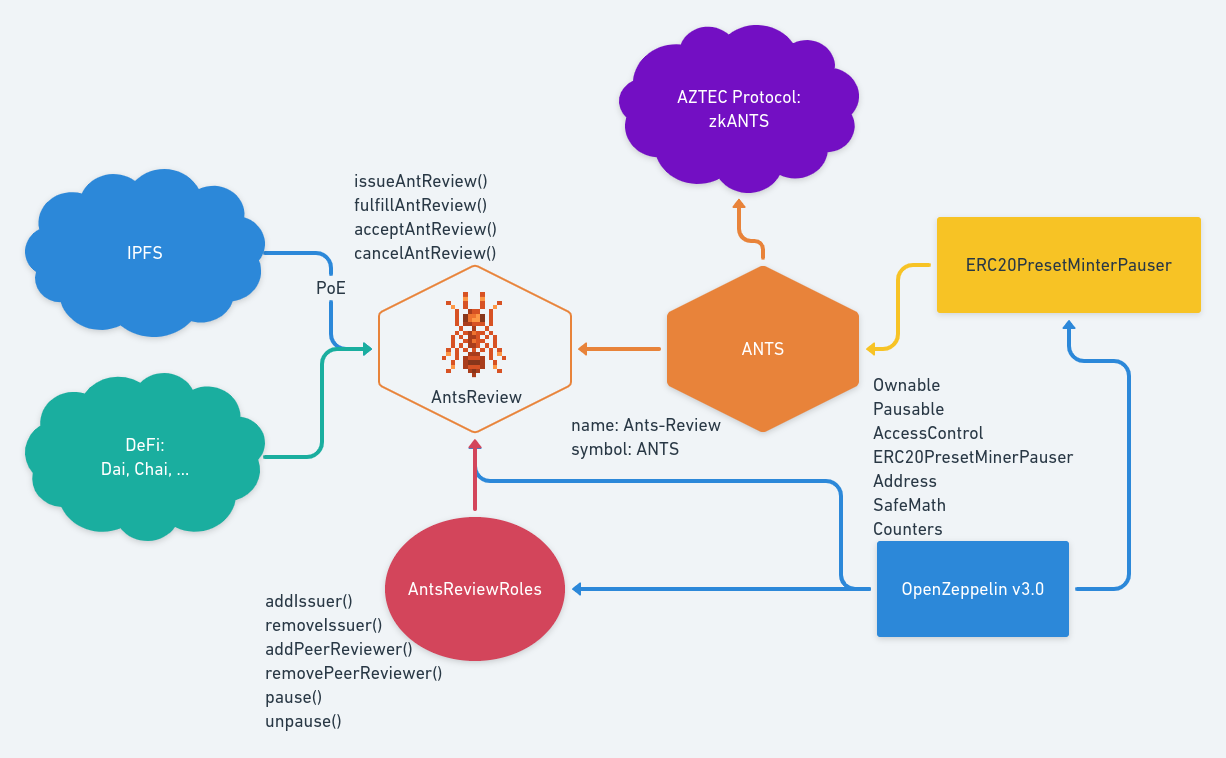
\includegraphics[scale=0.28]{AntsReview}
\caption{Ants-Review Smart Contracts}
\label{fig:contracts}
\end{figure}

In the following sections we describe the architecture of the system and its building blocks. 
\newline The Ants-Review Protocol is divided into different modules responsible for the following functionalities as shown in the flow-chart [Fig. \ref{fig:contracts}]:

\begin{itemize}
\item \emph{AntsReview}, which manages access management and the core system.
\item \emph{Tokenomics}, which manages the incentivization mechanism of the system.
\item \emph{Privacy}, which maintains the pseudo-anonymity of the system via AZTEC Protocol.
\end{itemize}

\subsubsection{AntsReview}
AntsReview is the core of the smart contracts written in Solidity \cite{Solidity}, an object-oriented programming language for writing smart contracts that runs on the Ethereum Virtual Machine (EVM), deployed on Ethereum Rinkeby's Testnet \cite{Rinkeby}.
\newline It implements a bounty-like system (AntReview) where an issuer (author or editor) is asked a series of actions to ensure transparency and consistency for the AntReview that he/she is creating:
\begin{itemize}
  \item to upload the file containing the requirements of the peer-review and the paper into IPFS\cite{IPFS}.
  \item to specify a deadline in the form of a unix timestamp after which the fulfillment will no longer be accepted.
  \item to send the amount of ether for the reward.
\end{itemize}

AntsReviewRoles, to ensure integrity of the system, implements an access management, leveraging on \emph{AccessControl.sol} by OpenZeppelin Solidity Library \cite{OZ}, through the creation of the Issuer and Peer-Reviewer Roles.
\newline It also integrates a circuit breaker design pattern via \emph{Pausable.sol} by OpenZeppelin to allow the Pauser Role, that by default is the Owner of the smart contracts, able to pause (or unpause) the functions in case of a security emergency, like an attack to the smart contracts. In this way, only the Issuer can create a new AntReview.
\newline Once created, an AntReview is available to be fulfilled by Peer-Reviewers, uploading the peer-review on IPFS before the deadline.When the AntReview is accepted by the Issuer, the bounty is paid among Peer-Reviewers.On top of that, the Issuer can cancel the AntReview at any time and withdraw the amount of ether staked.
\newline One of the key aspects of the protocol is the concept of Proof of Existence, introduced by Stuart Haber \& W. Scott Stornetta \cite{TimeStamp-Haber}. Pioneers of the blockchain, cited by the Bitcoin whitepaper\cite{Bitcoin}, they were on a mission to solve the problem of immutability of digital records that became reality with the Blockchain and Bitcoin as its first application. In Ethereum \cite{Ethereum} the concept of immutability is achieved via the blockchain and the proof of work consensus algorithm by a chain of timestamped block merkle tree root hashes that are secured by miners competing computations.
\newline Ants-Review exploits the advantages of storing the hashes of the peer-reviews into a Merkle Tree \cite{BayerHaber1992} to achieve immutability and efficiency in verifying the data with a complexity of O(logn) for searching through the tree.
\newline A Merkle tree is a particular type of binary tree, formed by a set of nodes with a large set of leaf nodes at the bottom of the tree representing the hash of the original data, a set of intermediate nodes where each node is the sum of the two children hashes, ending with a single root hash. In order to verify if a specific hash is included into a Merkle Tree by leveraging on \emph{MerkleProof.sol} (OpenZeppelin Library), we need to provide a proof, generated from the leaf of interest, that represents the ramification derived from the leaf, the root hash and, finally, the leaf we want to verify.
\newline The paper and peer-review documents will be included into a Merkle Tree by hashing the data using keccak256, a cryptographic hashing algorithm available in Solidity.

\subsubsection{Tokenomics}
AntsReview integrates few tokens, each of which plays an integral role in the functioning and anonymity of the decentralized protocol.
\newline ANTS, is the primary protocol token and can be staked into an AntReview.
\newline ANTS [see \ref{lst:code}] is implemented by inheriting \emph{ERC20PresetMinterPauser.sol} from OpenZeppelin Library with name \emph{Ants-Review} and symbol \emph{ANTS}.

\begin{lstlisting}[caption={ANTS.sol},label={lst:code},language=Solidity]
/// SPDX-License-Identifier: GPL-3.0
pragma solidity 0.6.8;

///@title Ants-Review
///@author Nazzareno Massari
///@notice ANTS ERC20 Token
///@dev All function calls are currently implemented without side effects through TDD approach
///@dev OpenZeppelin library is used for secure contract development

import "@openzeppelin/contracts/access/Ownable.sol";
import "@openzeppelin/contracts/presets/ERC20PresetMinterPauser.sol";


contract ANTS is Ownable, ERC20PresetMinterPauser {

  constructor()
  ERC20PresetMinterPauser("Ants-Review", "ANTS")
  public {

  }

}
\end{lstlisting}

\subsubsection{Privacy}
The anonymity of an agent in the system is achieved in two ways:

\begin{itemize}
  \item via pseudo-anonimity granted through Ethereum's Externally Owned Accounts (EOA) addresses that can pseudo-obscure the identity of the agent.
  \item via private transactions allowed by AZTEC Protocol security layer via zkANTS. Future developments will allow to leverage on PLONK\cite{PLONK}proofs, a universal ZK-SNARK construction, to reduce gas costs and improve scalability.
\end{itemize}

 Externally Owned Accounts (EOA) in Ethereum are controlled by private keys, are 20 bytes long and have no code. An user can send messages from an externally owned account by creating and signing a transaction. The limitation of this type of solution concerning the protocol's privacy is due to the fact that blockchain and transactions are public, therefore the details of transactions are visible to anyone by browsing a block explorer (like Etherscan), and are subjected to data mining that could extract value and identify users in the blockchain.
\newline To avoid that, Ants-Review will implement zkANTS, an Ant token wrapped into AZTEC Protocol. In the future zkANTS could leverage on zkSNARKS and PLONK, allowing private transactions in the system to maintain the privacy and anonymity of Peer-Reviewers.
\newline The AZTEC Protocol was conceived to enable privacy on public blockchains. It uses a series of zero-knowledge proofs (ZK-SNARKs) and homomorphic encryption to validate encrypted transactions.
\newline ZK-SNARKs (Zero-Knowledge Succinct Non-Interactive Argument of Knowledge) \cite{ZKSNARKs} refers to a proof construction where one can prove possession of certain information, like a secret key, without revealing that information, and without any interaction between prover and verifier.
\newline Zero-Knowledge \cite{ZeroKnoledge} proof is a mathematical cryptographic method that through value permutations allow one party (the prover) to prove to another (the verifier) the validity of a statement, without revealing the statement itself.
\newline Future developments will investigate viable solutions, for scaling the system, like ZK-Rollups by AZTEC Protocol, one of the options being developed for a type of layer 2 construction that runs on top of Ethereum to improve scalability. This will enable to run smart contracts at scale with quasi-instant transactions while still being secured by Ethereum.

\section{Discussions}
In this session we discuss future developments not yet implemented and implications of AntsReview.
\subsection{Possible developments}
An AntReview, issued by an author would be seen as a poll, a container where Anters (members of the Ants-Review Community) can stake ether or ERC20 tokens from DeFi services including Dai \cite{Dai}, Chai \cite{Chai}, ... with the possibility to accrue interest for the duration of an AntReview (1 year on average), via MakerDAO DSR (Dai Saving Rate) \cite{DSR} or Compound \cite{Compound} to cite a few.
 An AntsReview DAO could be formed in the future to allow ANTS stakers the ability to participates in a Decentralized Autonomous Organization which will be used to govern important aspects of the decentralized protocol, from smart contracts upgrades to more minor changes in settings across the protocol.
\newline Hive. When Anters make a deposit into an AntReview, they will instantly receive the Hive token which represents their deposit and the accrued interest it gains over time in the AntReview.
\newline This token doesn't need to be locked in the network and it can be traded, sold, or held as the Anter desires.
\newline Hive will be implemented using a similar approach to Chai, an ERC20 token that accrues interest from MakerDAO's DSR or Compound, with name \emph{Hive} and symbol \emph{HIVE}
\newline Ideally, but is still under investigation, after the deadline of the AntReview is reached, the Hive token will be burned for ANTS and wrapped into zkANTS to promote anonymity and sent between the peer-reviewers that fulfilled the AntReview.
\newline zkANTS, is an Ants-Review token wrapped into AZTEC Protocol \cite{AZTEC} ZK-SNARKs, that will be extended to PLONK \cite{PLONK} Proof to collapse the gas costs of private transactions on mainnet.
\newline zkANTS will be implemented via AZTEC 2.0 (still in development) that will allow to securely wrap the Ants-Review Token into zkANTS, allowing private transactions on mainnet and preserving the anonymity of Peer Reviewers.
\newline Finally, another concept under investigation is Quadratic Funding \cite{LiberalRadicalism}, used by Gitcoin \cite{Gitcoin} to match donations for Grants. This will allow to incentivise prolific Peer-Reviewers and improve the stability of the system together with ideally a reward system to rank the best Peer-Reviewers.

\subsection{Criticism}
Some criticism towards giving a monetary reward to reviewers tackle the fact that an extrinsic motivation (such as a token system) might decrease the intrinsic motivation that drives researchers to perform scientific contributions. Some experimental studies seem indeed to suggest that reviewers are more interested in reputational forms of recognition \cite{Warne-RewRev,ZahIncent} and that material compensation affects the quality of reviews by 'undermining the moral motives that guide referees' behaviour \cite{SquazzIncent}. However, we think that engaging the whole community towards the peer-review process and rewarding each actor in it through gamified forms of reward and alternative voting systems could diminish these effects, but this is a speculation that needs to be experimentally tested.

\subsection{A new community-driven standard?}
As Tennant points out\cite{Tennant2017-F1000R}, a change is already happening in the publishing industry, especially with new born publishers opening up the review process (BioMed Central, ELife, Frontiers, PeerJ, F1000 Research). If also pre-print platforms integrate peer-review into their platforms, the dissociation of initial scientific dissemination and scientific validation will force publishing industry to adapt in order to justify their added value.
In our proposal we posed two possible integrations for Ants-Review, a simpler one which maintains part of the journals' power in the peer-review evaluation and more complex one that completely decouples the peer-review process from the publishers giving it back to the scientific community and applying concepts from mechanism design. This second option, which requires further implementations, is the one we aim at. Indeed, we foresee that the future will evolve towards community-organized peer reviews: peer reviews will be more and more independent from publishers, and researchers will be the ones seeking the papers to review with a reputation build within community and not journals.
Peer reviews requires a standard: building smart-contracts for peer-reviews might set a first step in this direction and our work seems promising. We hope that soon the value of peer review as 'academic capital' will be recognized by research funders and hiring committees.

\section{Conclusion}
In this paper we addressed a crucial problem within scholarly academic communication: the peer-review process. We've shown how blockchain technology could provide an efficient and viable solution to open up possible directions for a paradigm shift in scientific communication. We proposed an incentive mechanism that could solve the problems of lack of acknowledgment and trust during peer-reviews. We exposed the architecture of our project for which we adopted cutting-edge tools from the open source blockchain ecosystem.

\subsubsection{Supplementary material}
Source Code, DOI: 10.5281/ZENODO.3829162
\newline Demo (PoC), DOI: 10.5281/ZENODO.3829183

\subsubsection{CRediT Authorship Contribution Statement}
 Bianca Trovò: Conceptualization, Investigation, Design, Writing - original draft, Writing - review \& editing. Nazzareno Massari: Project administration, Design, Software development, Visualization, Writing - review \& editing. Both authors equally contributed and supervised the project.

\subsubsection{Declaration of Competing Interest}
The authors declare no competing interests.

\subsubsection{Acknowledgements} We would like to thank Matteo A. Tambussi and Keno Budde for useful comments and discussions and Marcelo Colmenero for the Pixel Art.


% ---- Bibliography ----
%
% BibTeX users should specify bibliography style 'splncs04'.
% References will then be sorted and formatted in the correct style.
%
\bibliographystyle{splncs04}
\bibliography{ref1-intro.bib,ref2-peerreview.bib,ref2-relatedwork.bib, ref3-system.bib,ref4-discuss.bib, ref5-extra.bib}

\end{document}
